\documentclass[10pt]{beamer}
\setbeamertemplate{navigation symbols}{}

\setbeamercolor{frametitle}{fg=black,bg=red}
\setbeamercolor{title}{fg=black,bg=white!85!orange}
\usetheme{CambridgeUS}

\usepackage[russian]{babel}
\usepackage[utf8]{inputenc}
\usepackage{listingsutf8}
\usepackage{algorithm}
\usepackage{algpseudocode}
\usepackage{tcolorbox}

\usepackage{array}
\usepackage{multirow}

\lstloadlanguages{[Auto]Lisp}

\lstdefinestyle{base_listing}{
  extendedchars     = {true},
  inputencoding     = {utf8}, 
  basicstyle        = {\ttfamily \scriptsize},
  keywordstyle      = {\rmfamily \bfseries},
  commentstyle      = {\rmfamily \itshape},
  tabsize           = {2},
  flexiblecolumns   = {false},
  showstringspaces  = {falsedany},
  breaklines        = {true}, 
  breakatwhitespace = {true}
}

\definecolor{lred}{rgb}{1,0.78,0.79}
\definecolor{lgreen}{rgb}{0.9,1,0.8}


\lstdefinestyle{base_listing_floating}{
  style   = {base_listing},
  numbers = {none},
  % float = {h}, % float right where we put it
  % aboveskip = 0pt, 
  % belowskip = 0pt
}


\lstdefinestyle{crs_cpp}{
  style    = {base_listing},
  language = {C++}
}


% очень бедное определение ассемблера LLVM для листингов
% выделены только ключевые слова, встречающиеся в примерах
\lstdefinelanguage{LLVM-asm}
{
  morekeywords = {
    load, store, malloc, alloca, free, getelementptr,
    add, sub, insertvalue, extractvalue, icmp, call
  },
  sensitive   = false,
  morecomment = [l]{;}
}

\lstdefinestyle{crs_llvm}{
  style    = {base_listing_floating},
  language = {LLVM-asm}
}


\beamersetuncovermixins{\opaqueness<1>{25}}{\opaqueness<2->{15}}
\begin{document}
\title[Scheduler]{Разработка и встраивание планировщика в ОС Linux}
\author[Степанов Даниил]{Студент: Степанов Даниил}
\institute[]{Санкт-Петербургский политехнический университет Петра Великого}
\date{\today} 


\begin{frame}
\titlepage
\end{frame}

%\begin{frame}\frametitle{Table of contents}\tableofcontents
%\end{frame} 


\begin{frame}\frametitle{Планирование}
Политики планирования ядра 2.6:
\begin{itemize}
\item SCHED\_NORMAL
\item SCHED\_FIFO 
\item SCHED\_RR 
\end{itemize}
\end{frame}

\begin{frame}\frametitle{SCHED\_EDF}
SCHED\_EDF - это планировщик ЦП в реальном времени, который:
\begin{itemize}
\item позволяет указать временные ограничения для каждой задачи
\item построен вокруг концепции резервирования ресурсов
\item основан на хорошо известных алгоритмах планирования 
\end{itemize}
\end{frame}

\begin{frame}\frametitle{SCHED\_EDF}
Задача характеризуется следующими параметрами:
\begin{itemize}
\item время готовности
\item наихудшее время выполнения
\item дедлайн 
\end{itemize}
\end{frame}

\begin{frame}\frametitle{Earliest deadline first}
\center
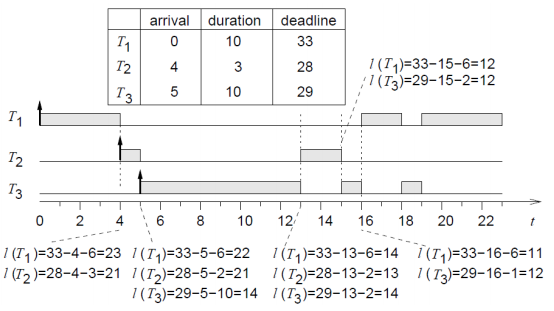
\includegraphics[width=10cm, height=10cm,keepaspectratio]{sched6}
\end{frame}

\begin{frame}\frametitle{Для чего полезна SCHED\_EDF}
Политика устанавливается для достижения двух результатов:
\begin{itemize}
\item гаратии времени
\item ограничения сроков
\end{itemize}
\end{frame}

%\begin{frame}\frametitle{Реализация}
%\begin{lstlisting}
%#ifdef	CONFIG_SCHED_EDF_POLICY
%#define SCHED_EDF		6
%#endif
%\end{lstlisting}
%\end{frame}

\begin{frame}[fragile]\frametitle{Реализация EDF}
\center
	\begin{columns}
		\column{0.5\textwidth}
		\begin{lstlisting}[style=crs_cpp]
		
struct edf_task{
	struct rb_node edf_rb_node;
	unsigned long long absolute_deadline;
	struct list_head edf_list_node;
	struct task_struct *task;
};
 		\end{lstlisting}
 		
		\column{0.5\textwidth}
		\begin{lstlisting}[style = crs_llvm]
struct edf_rq {
	struct rb_root edf_rb_root;
	struct list_head edf_list_head;
	atomic_t nr_running;
};
 		\end{lstlisting}
 	\end{columns}
\colorbox{white}{\parbox{0.9\textwidth}{{\begin{center}  \end{center} }}}\\

\end{frame}

\begin{frame}\frametitle{}
Чтобы добавить новую политику планирования в ядро Linux, необходимо создать новый модуль
\center
\includegraphics[width=8cm, height=8cm,keepaspectratio]{sched8}
\end{frame}


\begin{frame}[fragile]\frametitle{}
Согласно модульным правилам планирования, каждый модуль должен реализовывать набор функций, указанных в структуре sched\_class
\center
	\begin{columns}
		\column{0.9\textwidth}
		\begin{lstlisting}[style=crs_cpp]
		

const struct sched_class edf_sched_class = {
	.next 			= &rt_sched_class,
	.enqueue_task		= enqueue_task_edf,
	.dequeue_task		= dequeue_task_edf,

	.check_preempt_curr	= check_preempt_curr_edf,

	.pick_next_task		= pick_next_task_edf,
	.put_prev_task		= put_prev_task_edf,

	.set_curr_task          = set_curr_task_edf,
	.task_tick		= task_tick_edf,
};. 
 		\end{lstlisting}
 	\end{columns}
\colorbox{white}{\parbox{0.9\textwidth}{{\begin{center}  \end{center} }}}\\
\end{frame}


\begin{frame}[fragile]\frametitle{}
Изменения в sched.c для включения файла, реализующего модуль EDF:
\center
	\begin{columns}
		\column{0.9\textwidth}
		\begin{lstlisting}[style=crs_cpp]
		

#include "sched_rt.c"
#ifdef CONFIG_SCHED_DEBUG
#include "sched_debug.c"
#endif
#ifdef	CONFIG_SCHED_EDF_POLICY
#include "sched_edf.c"
#endif

#ifdef	CONFIG_SCHED_EDF_POLICY
	#define sched_class_highest (&edf_sched_class)
#else
	#define sched_class_highest (&rt_sched_class)
#endif

 		\end{lstlisting}
 	\end{columns}
\colorbox{white}{\parbox{0.9\textwidth}{{\begin{center}  \end{center} }}}\\
\end{frame}

\begin{frame}[fragile]\frametitle{}
Чтобы задать требуемые параметры планирования задачи, необходимо изменить структуру данных struct sched\_param:
\center
	\begin{columns}
		\column{0.9\textwidth}
		\begin{lstlisting}[style=crs_cpp]
struct sched_param {
	int sched_priority;

#ifdef	CONFIG_SCHED_EDF_POLICY
	unsigned int	edf_id;
	unsigned long long deadline;
#endif
 };
 		\end{lstlisting}
 	\end{columns}
\colorbox{white}{\parbox{0.9\textwidth}{{\begin{center}  \end{center} }}}\\
\end{frame}


\begin{frame}\frametitle{Реализация SCHED\_EDF}
Дополнительные изменения:
\begin{itemize}
\item Включение политики в исходную функцию ядра rt\_policy 
\item sched\_setscheduler
\item \_setscheduler 
\end{itemize}
\end{frame}

\begin{frame}\frametitle{Сборка и встраивание ядра}
\begin{itemize}
\item С помощью утилиты wget загружаем исходный код ядра
\item Распаковываем архив
tar –xjvf linux-2.6.24.tar.bz2
\item Создаем конфигурационный файл из текущего системного конфигурационного файла:
sudo cp /boot/config-2.6.24 .config
\item Меняем параметр extraversion в Makefile, чтобы отличать собираемое ядро от других версий
EXTRAVERSION= -edf
\item Применяем патч:
patch -p1 < ../sched.patch
\item Компилируем ядро: \\
sudo make oldconfig \\
sudo make-kpkg –initrd kernel\_image 2>../errors
\item Начинается компиляция ядра, и если все идет хорошо, создается сжатый образ ядра
\item Установим скомпилированную версию ядра, сгенерированную предыдущим шагом
sudo dpkg -i kernel\_image-2.6.24\_xxxx.deb
\end{itemize}
\end{frame}

\begin{frame}[fragile]\frametitle{Тестирование}
\begin{itemize}
\item Был применен патч и встроено новое ядро
\item Написан код, устанавливающий процессу новую политику планировки
\item Написан код, устанавливающий процессу политику планировки SCHED\_DEADLINE в ядре 3.16
\end{itemize}
\center
	\begin{columns}
		\column{0.5\textwidth}
		\begin{lstlisting}[style=crs_cpp]	
[1455]
missed deadlines  = 2856
missed periods    = 821
Total adjustments = 48064 us
deadline   : 1000 us
runtime    : 400 us
nr_periods : 6368
 		\end{lstlisting}
 		
		\column{0.5\textwidth}
		\begin{lstlisting}[style = crs_llvm]
[1460]
missed deadlines  = 3802
missed periods    = 1026
Total adjustments = 20386 us
deadline   : 1000 us
runtime    : 400 us
nr_periods : 5188
 		\end{lstlisting}
 	\end{columns}
\colorbox{white}{\parbox{0.9\textwidth}{{\begin{center}  \end{center} }}}\\
\end{frame}




\end{document}